\subsection{Environments}
For our experiments, we choose environments provided by \textit{OpenAI Gym} \cite{gym}, which is a toolkit for developing and comparing reinforcement learning algorithms. It provides us with a simple and easy to use environment interface and a wide range of environments to develop general-purpose agents.

More specifically, we choose two of the environments shipped with OpenAI Gym, namely \textit{CartPole-v1} and \textit{LunarLander-v2}, shown in Figure \ref{fig:environments}. These environments are relatively iconic in the reinforcement learning community and, due to their simplicity, the learning progress and pitfalls can be easily understood by a human.
\begin{figure}[b]
    \centering
    \begin{subfigure}{0.49\textwidth}
        \raggedleft
        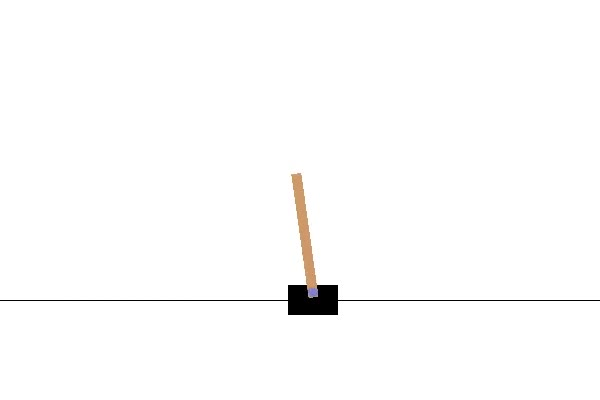
\includegraphics[width=\textwidth]{assets/cartpole.jpg}
    \end{subfigure}
    \begin{subfigure}{0.5\textwidth}
        \raggedright
        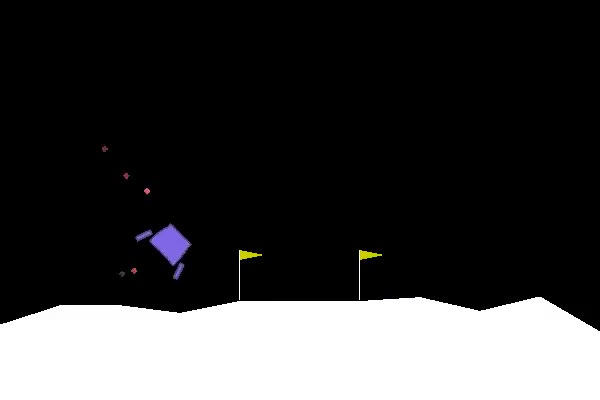
\includegraphics[width=\textwidth]{assets/lunarlander.jpg}
    \end{subfigure}
    \caption{Screenshots of the CartPole-v1 (left) and LunarLander-v2 (right) OpenAI Gym environments \cite{gym}.}
    \label{fig:environments}
\end{figure}
A more meaningful benchmark would include significantly more complex environments, such as Chess, Go, and Atari games, as was done for the original MuZero agent. Furthermore, experiments with robot agents, like a robotic arm grasping for objects, could demonstrate real-world viability for the algorithms. Unfortunately, due to MuZero's high computational requirements, we are unable to properly test these environments with various hyperparameters and achieve sufficient statistical significance. The exploration of more demanding environments is therefore left to future work.

In CartPole-v1, the agent controls a cart that can only move horizontally on one axis. Attached to the cart is a pole that starts off relatively upright and can spin freely around the horizontal axis perpendicular to the cart's movement. The goal is to balance the pole as long as possible so that it never exceeds $15$ degrees from being perfectly vertical. Moving the cart too far to the left or right (i.e. out of bounds) also results in episode termination. Only two actions are available, namely the acceleration in either direction, and a reward of $1$ is given for each timestep foregoing termination, up to a maximum of $500$ steps.

The objective in the LunarLander-v2 environment is, as the name suggests, to safely land a lander on the moon's surface. This is done by controlling three thrusters: The main engine, and two orientation rockets. Various rewards are given to incentivize the agent to pursue this behavior, such as a bonus for approaching the landing pad, and a small negative penalty for using the main engine, encouraging fuel efficiency. Perhaps most notably, however, a large negative reward of $-100$ is given for crashing the lander.